% !TeX spellcheck = en_GB
\documentclass{article}
\usepackage{graphicx}
\usepackage{lmodern}
\usepackage[T1]{fontenc}
\usepackage{hyperref}
\usepackage{textcomp}
\hypersetup{
	colorlinks=true,
	linkcolor=blue,
	filecolor=magenta,      
	urlcolor=cyan,
}
\begin{document}
\begin{center}
	\underline{\LARGE IT Solutions }
\end{center}
\begin{center}
	\underline{ \LARGE Setting Up a Network }
\begin{figure}[h]
		\centering
		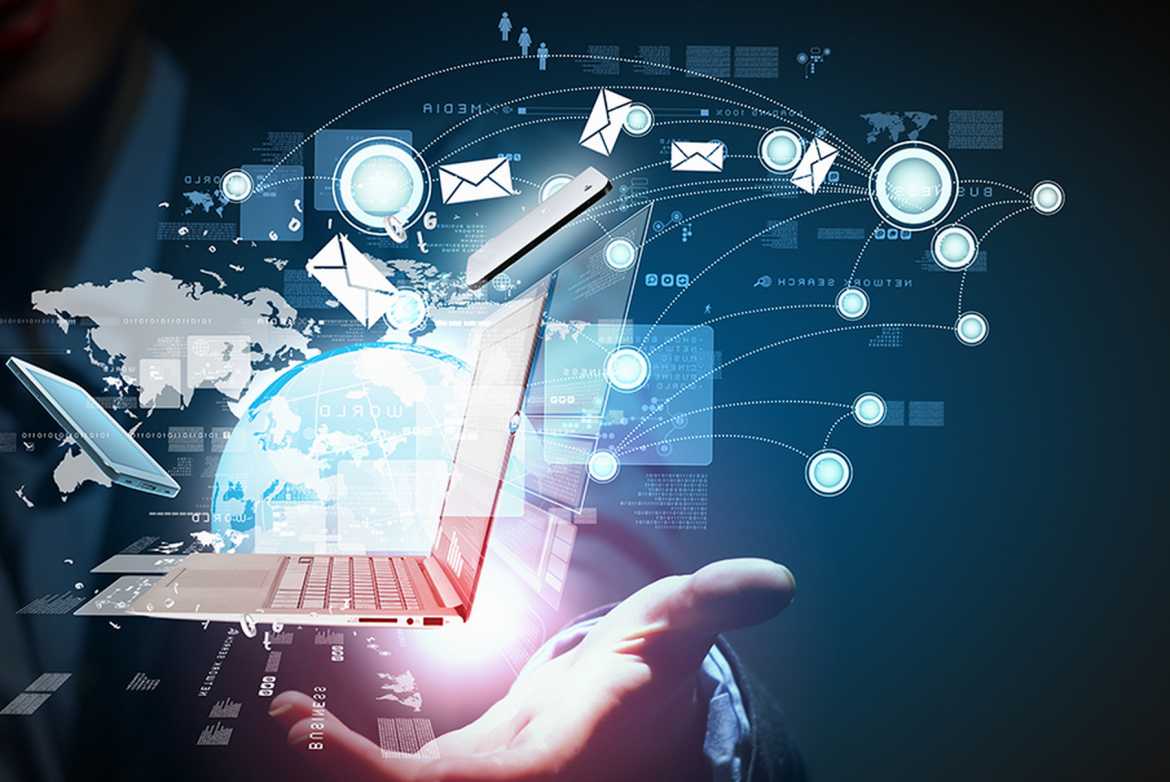
\includegraphics[width=1\textwidth]{1}
		\newline
		{Brett W, Sonja E, Allen P, Sydney K}
\end{figure}
\end{center}
	\pagenumbering{gobble}
	\newpage
		\pagenumbering{arabic}
	\tableofcontents
	\newpage
\section{Introduction}
	Our company was approached by SIIT to come up with a network solution that would efficiently suit their business requirements. They require implementation of multiple VLANs on the network to provide redundant reliable service to all their employees and clients. The network we will be implementing should consist of the following equipment: 6 routers, 4 switches, one primary domain controller, one backup domain controller, several windows client machines spread across the two subnets, at least three windows client machines set up in their own VLAN (for audio and video streaming), a Linux server running Clonezilla software, and two printers set up in the printer pool.  
	\newline\newline
	The purpose of multiple subnets is to make the network run a lot smoother, as well as split up the two VLANs: staff and student. The purpose of setting up the VLANs is so that remote end devices can still access all of the network resources they are required to access.\newline
	\newline\newline
	\newpage
\section{Network Sketch}
\begin{figure}[h]
		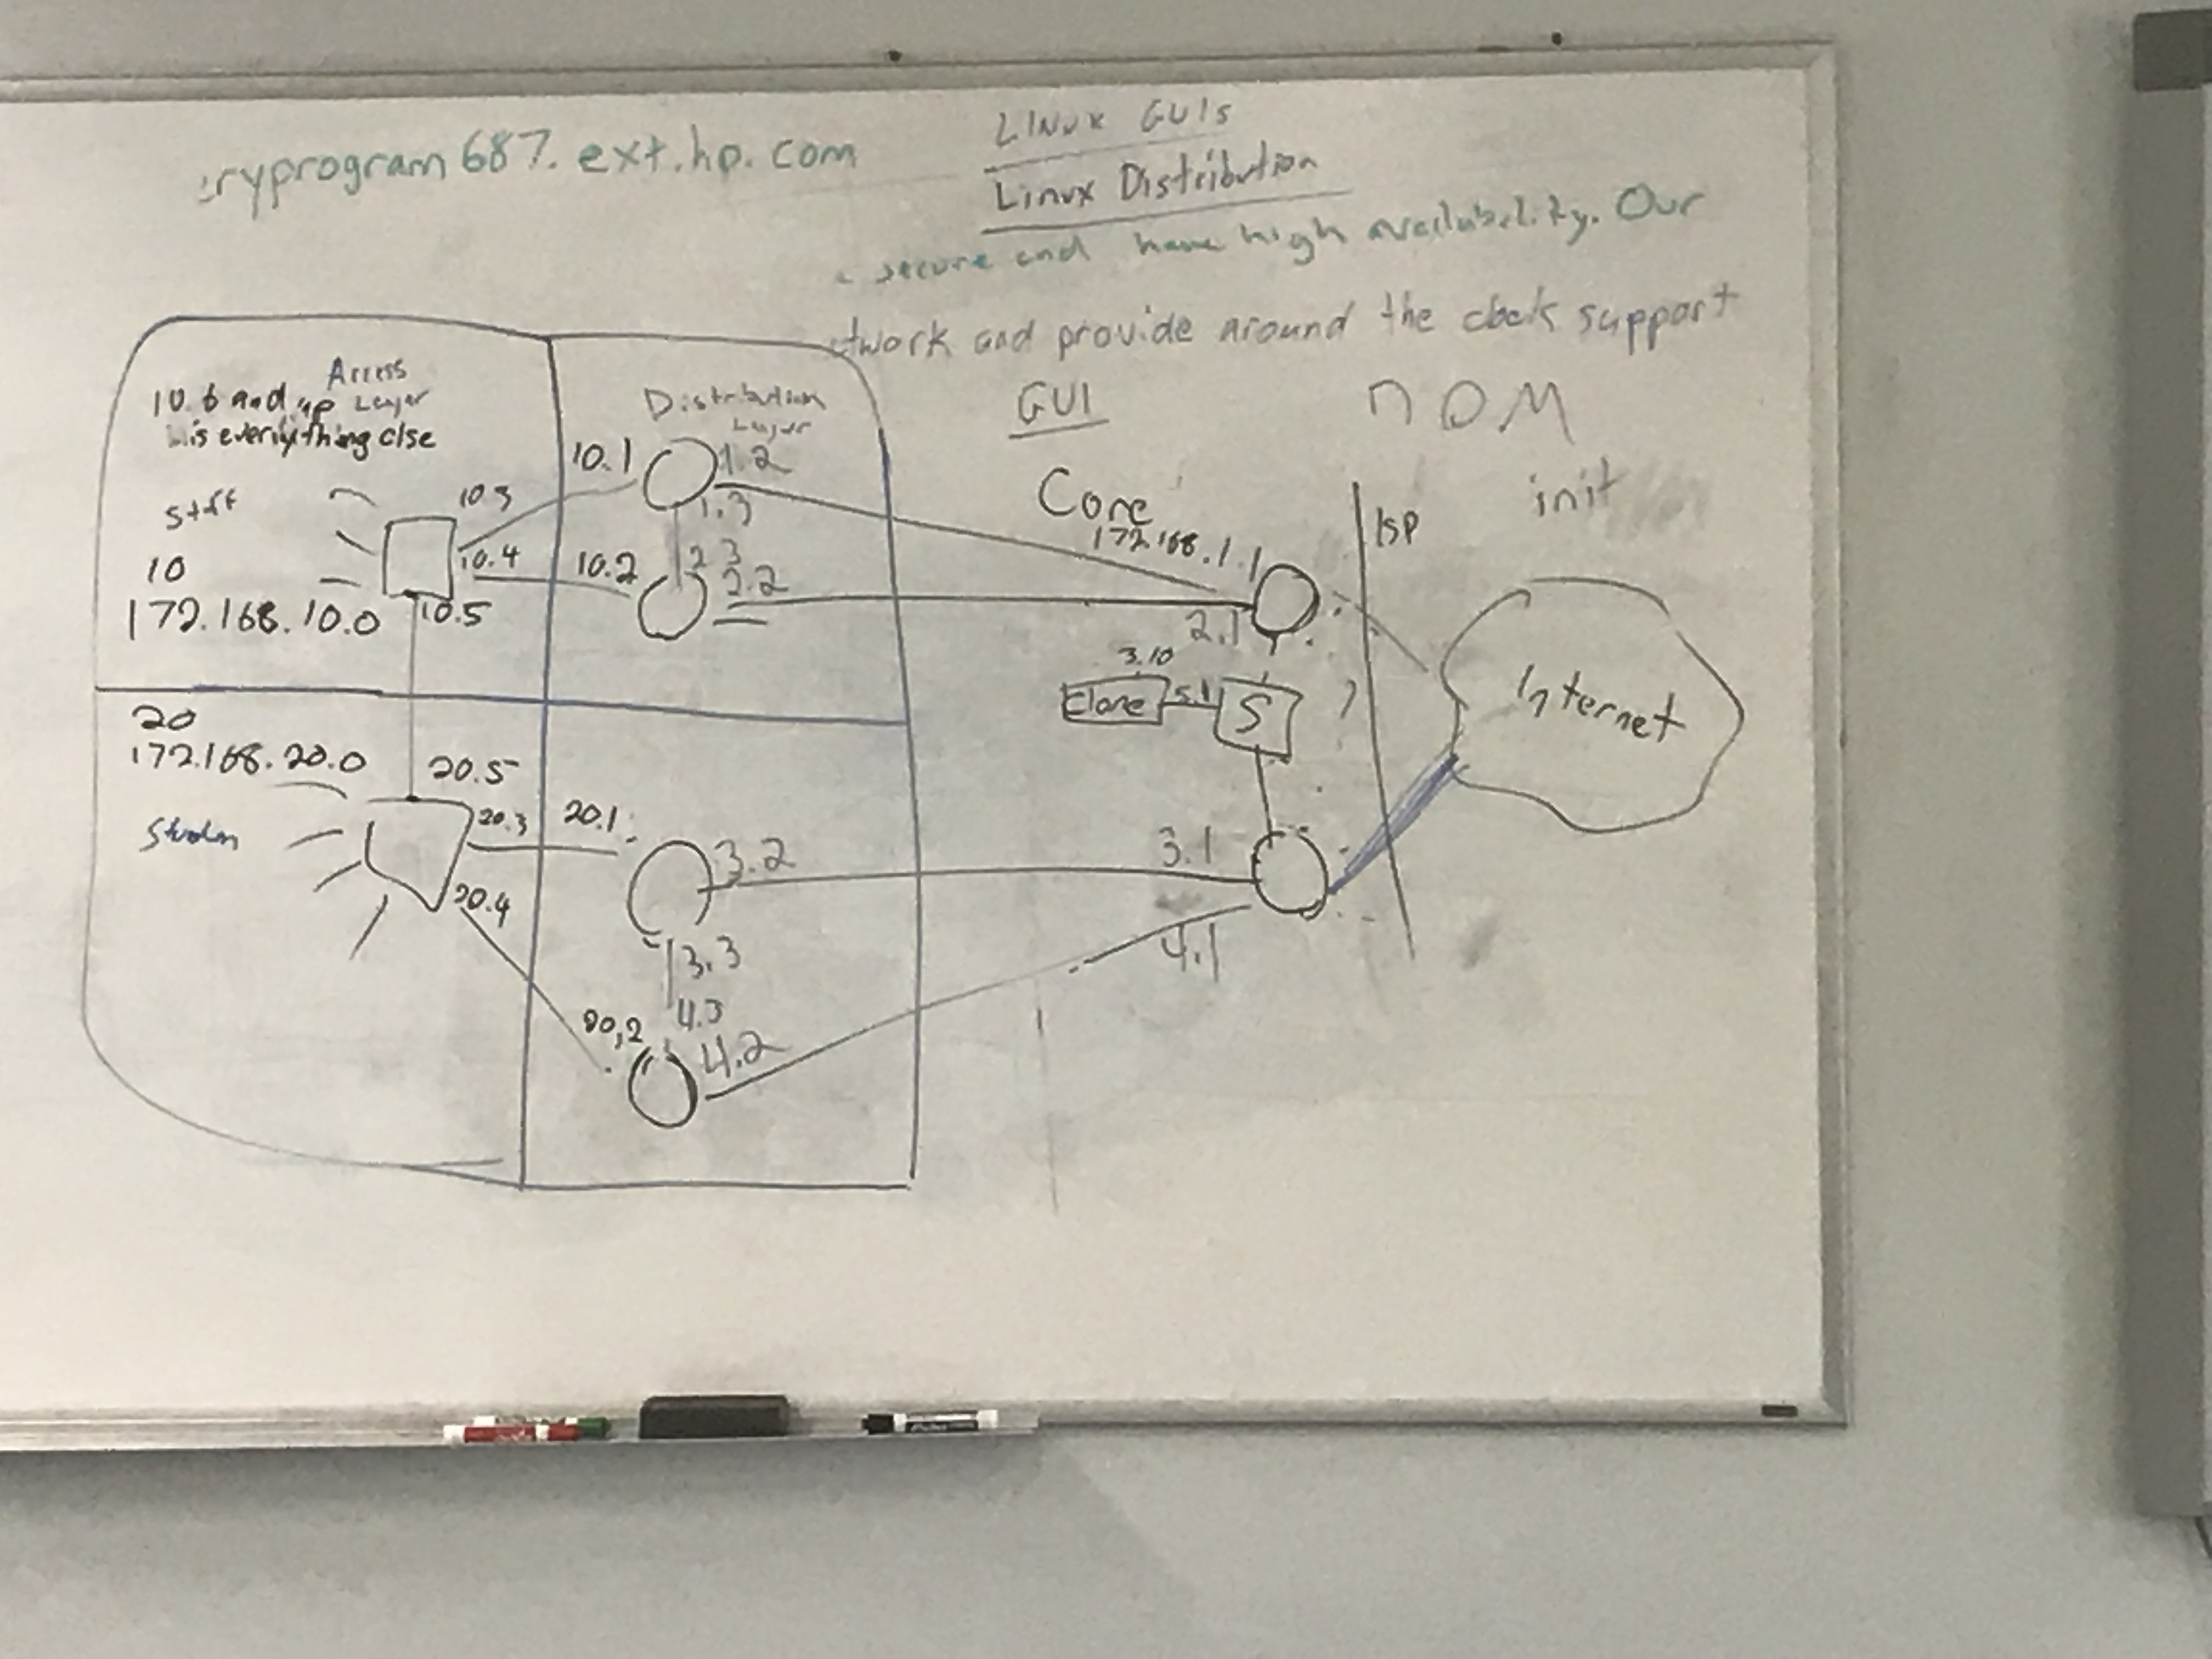
\includegraphics[width=1\linewidth]{2}
\end{figure}
	The network sketch will give you a rough idea of how you want the network to work and function. The sketch will show you how the topology would look before implementing it in a virtual environment. During the process, you should consider how much equipment will be needed and how much equipment you have access to.
	\newpage
\section{Network Map}
\begin{figure}[h]
		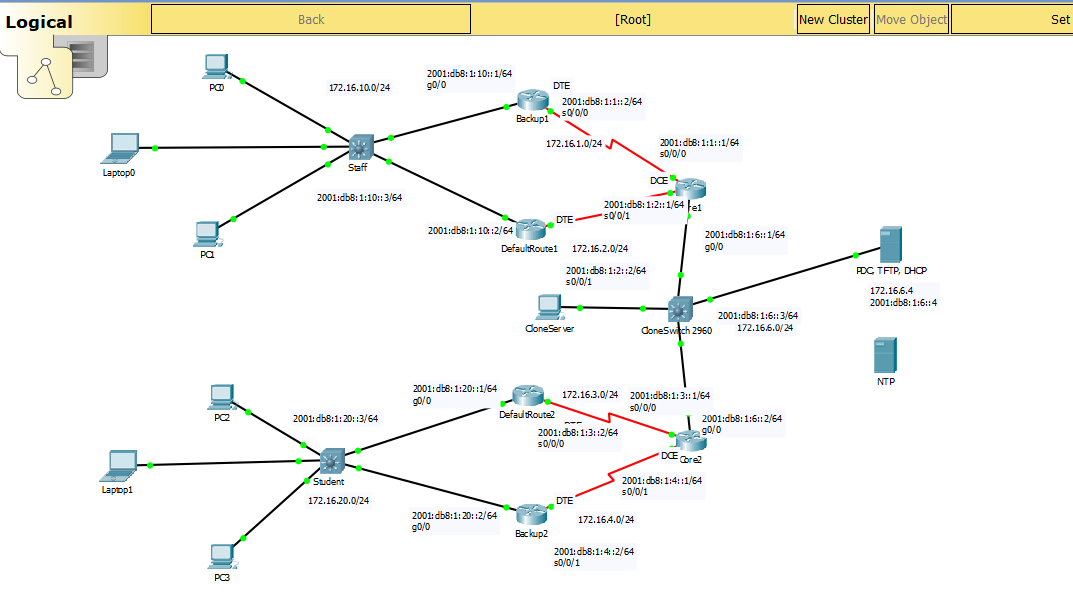
\includegraphics[width=1\linewidth]{3}
\end{figure}
	The network map is the implementation of the network sketch in a virtual environment such as Cisco Packet Tracer. In this environment you are able to assign IP addresses, routing protocols (OSPF, RIP, EIGRP, ISIS) and connect devices. This program also allows you to see the flow of packets throughout the network.
	\newpage
\section{IP Addressing Scheme}
\begin{figure}[h]
		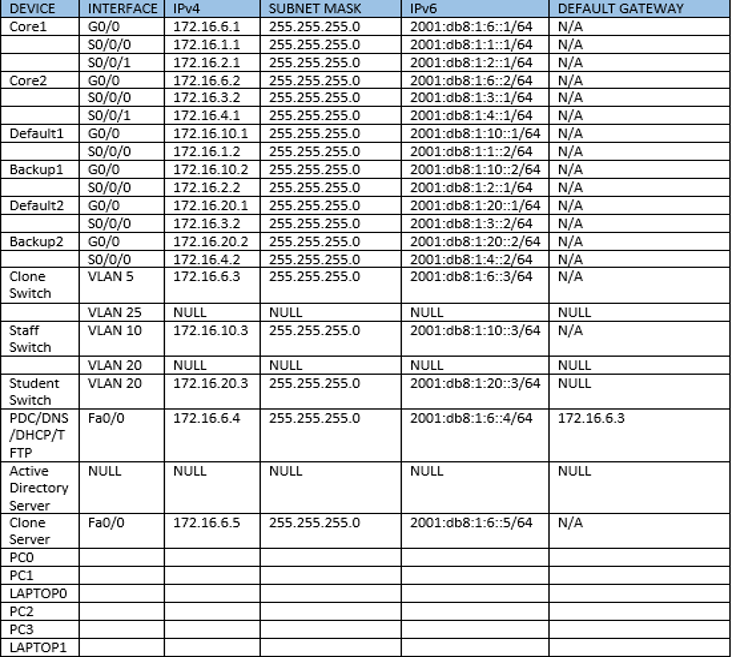
\includegraphics[width=1\linewidth]{4}
\end{figure}
	The IP addressing scheme is used to keep track of the addresses in your network. Without IP addresses devices would not have connectivity. There are two types of IP addresses: IPv4 (eg. 192.168.1.0/24) and IPv6 (eg. 2001:db8:acad::1/64).
	\newpage
\section{Preparing The Equipment}
\begin{figure}[h]
		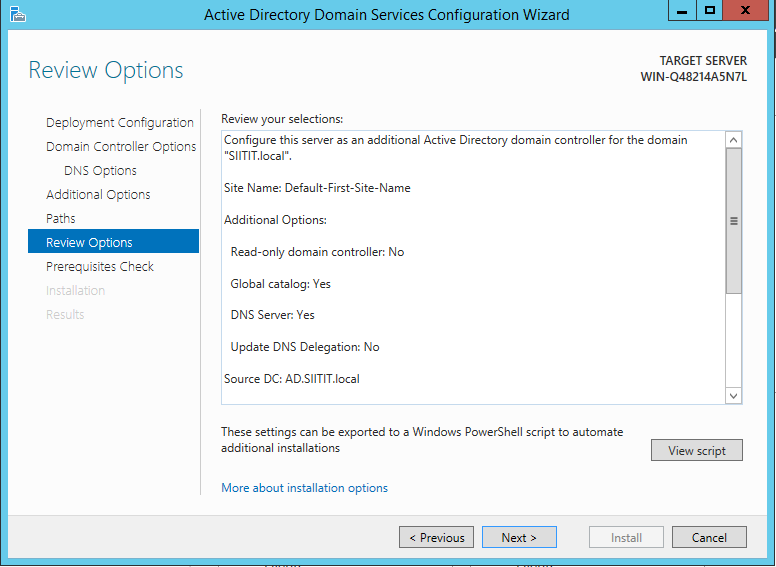
\includegraphics[width=1\linewidth]{5}
\end{figure}
	Before working on your equipment be sure to erase the startup configuration (erase startup-config) followed by the reload command (reload). This is done to restore the devices to default factory settings.
	\newpage
\section{Initializing the Devices}
\begin{figure}[h]
		\includegraphics[width=1\linewidth]{"staff passwords"}
\end{figure}
\subsection{Hostnames}
	Before you begin setting up and configuring a router or switch you want to set the hostnames. You set these hostnames so you can identify which device your connected to. 
\begin{figure}[h]
		\centering
		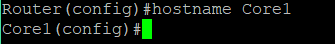
\includegraphics[width=0.5\linewidth]{hostname}
\end{figure}
\subsection{Password Encryption}
	When you first begin setting up a router or switch you want to make sure that the switch is password protected. By doing this you will not allow anyone access without a password. Using the "service password-encryption" command will take that password and encrypt it so that it will not be shown in plain text.
\begin{figure}[h]
	\centering
		\includegraphics[width=0.6\linewidth]{"staff password encryption"}
\end{figure}

\subsection{Telnet}
	Telnet is a simple, text-based network protocol that is used for accessing remote networks over TCP/IP networks. Telnet was created in 1969 and has been replaced by SSH because Telnet poses security issues.
\begin{figure}[h]
		\centering
		\includegraphics[width=0.5\linewidth]{"telnet access"}
\end{figure}
\newpage
\subsection{Message Of The Day}
	The banner Message of The Day(MOTD) is a message that is presented to someone who is access the router or the switch. Most network administrators use it to display legal notices regarding access to the device.
\begin{figure}[h]
	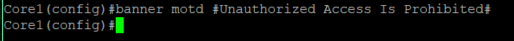
\includegraphics[width=1\linewidth]{motd}
\end{figure}
\subsection{Default Route}
The default route is a setting on a device that defines the packet forwarding rule to use when no specific route can be determined for a given Internet Protocol(IP) destination address.
\begin{figure}[h]
	\includegraphics[width=1\linewidth]{"default route"}
\end{figure}
\newpage
\section{Configure Device Ports}
An Internet Protocol (IP) address is a unique identifier that is assign to specific ports to allow communication between devices on a network. An IP address provides an identity to a networked device. There are 2 types of IP addresses IPv4 and IPv6, IPv6 is the successor to IPv4 and is less likely to run out of IP addresses. In order to use IPv6 addresses you have to enable unicast routing.
\begin{figure}[h]
	\centering
	\includegraphics[width=0.9\linewidth]{"configure ip address"}
\end{figure}
\begin{figure}[h]
	\centering
	\includegraphics[width=0.5\linewidth]{"enable ipv6 core1"}
\end{figure}
\subsection{Labelling Ports}
When a network administrator configures a description on a port it gives that interface a label of what the interfaces purpose is and what it is connected to.
\begin{figure}[h]
	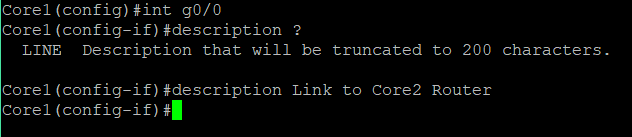
\includegraphics[width=1\linewidth]{description}
\end{figure}
\newpage
\subsection{Clock Rate}
The clock rate is important for routers because it defines which side of the WAN link is the DCE and what side is DTE. The clock rate sets the speed at which data is transferred over the network. If your clock rate is low then your bandwidth will be low.
\begin{figure}[h]
	\centering
	\includegraphics[width=0.5\linewidth]{"clock rate"}
\end{figure}
\subsection{Interfaces}
To activate an interface you can specify which interface or ranges of interfaces that you want to activate. If an interface is not activated then it will not be able to transfer data through it until the \textbf{no shutdown} command has been issued.
\begin{figure}[h]
	\centering
	\includegraphics[width=0.5\linewidth]{"activate interfaces"}
\end{figure}
\section{Test and Troubleshoot Network Connectivity}
Troubleshooting commands:
\newline
1: show running-config (Displays the entire routers configuration)
\newline
2: show ip interface brief (Displays information about the interface)
\newline
3: show ip(v6) route (Displays all available routes on your router)
\newline
4: show interfaces (Displays all interfaces with detailed information(interface speed,bandwidth, clock rate etc.)
\newline
5: copy running-config startup-confg (copies the current running configuration to the startup configuration)
\newline
6: ping 'ip-address' (Will verify connectivity between devices)
\newline
7: traceroute (Traces the routes packets take within the network to it's destination)
\newline
8: show ip(v6) ospf (Shows the number of interfaces in each area and the areas)
\newline
9: show ip(v6) protocols (Shows which routing protocol, router-id, and attached networks)
\newpage
\section{Setting up DHCP}
Dynamic Host Configuration Protocol(DHCP) is a network management protocol used on TCP/IP networks where a DHCP server dynamically assigns an IP address and other network configuration parameters to each device on a network so they can communicate with other IP networks.
\subsection{Installing DHCP}
To install DHCP run the following command.
\begin{figure}[h]
	\centering
	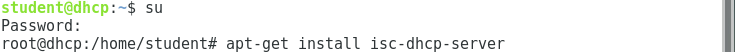
\includegraphics[width=1\linewidth]{dhcp-install}
\end{figure}
\subsection{Configuring DHCP}
\begin{figure}[h]
	\centering
	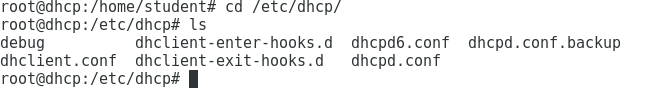
\includegraphics[width=1\linewidth]{dhcp-config1}
\end{figure}
Change the directory to /etc/dhcp\newline\newline
Using a text editor such as vi, vim, or nano you will need to edit the file: dhcpd.conf. Here you want to set up the subnets so that the hosts connected to those specific networks get an ip address in those ranges. For each zones in your network you'll need to specify the range of IP addresses, the subnet mask, default gateway and DNS servers.
\newpage
\begin{figure}[h]
	\centering
	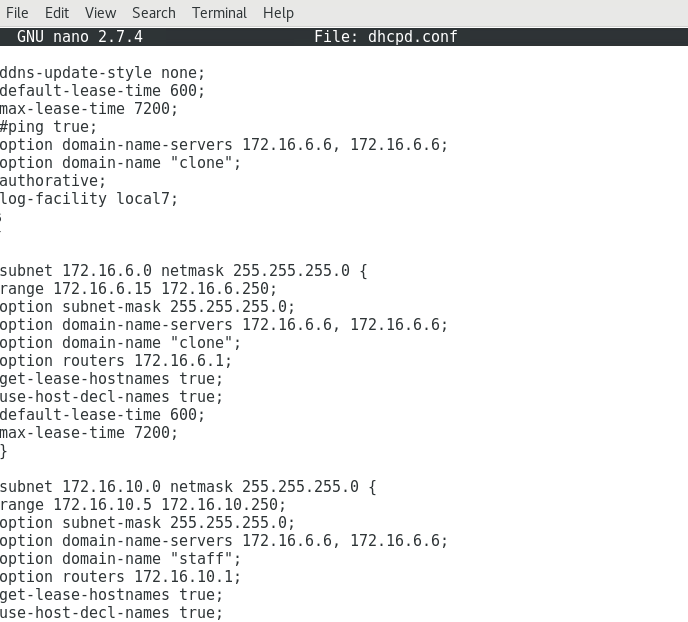
\includegraphics[width=1\linewidth]{dhcp-config2}
\end{figure}
\newpage
\begin{figure}[h]
	\centering
	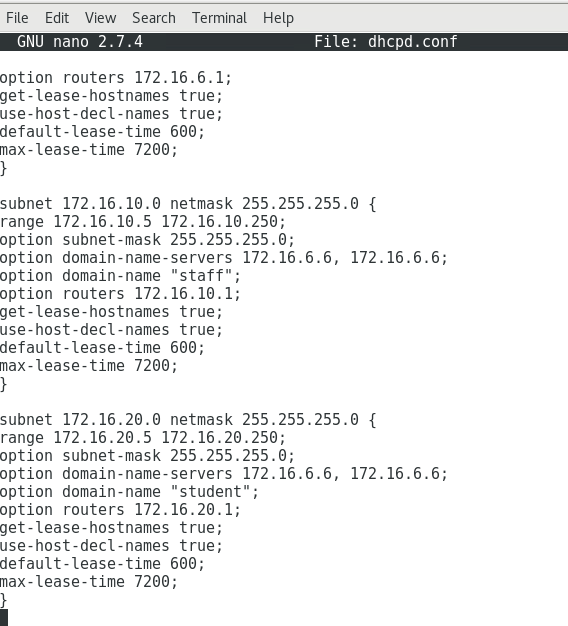
\includegraphics[width=1\linewidth]{dhcp-config3}
\end{figure}
\newpage
Running the following command restarts the DHCP server with the new settings in the configuration file.
\begin{figure}[h]
	\centering
	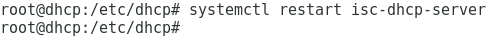
\includegraphics[width=1\linewidth]{dhcp-config4}
\end{figure}
	\section{Setting up the PDC and DNS}
	\label{sec:10.1}
The Primary Domain Controller (PDC) is the main service which controls all aspects of the domain including users, groups, and different services that the network may need.
The Domain Name System (DNS) is a central part of the Internet, it provides a way to match the name of a website to its IP address.
\subsection{Primary Domain Controller}
First step you need to do is install \textbf{Windows Server 2012} or equivalent.
Then follow these steps:
\begin{enumerate}
\item Click \textbf{Add Roles and Features} in the Server Manager.
\item Check the Active Directory Domain Services box.
\item Check the DNS Server box.
\item Click on Add Features for both of the services.
\item Click Next until you reach the confirmation window. 
\item Click install to begin your installation if all prerequisites have been met.
\item Restart your server after installation is complete.
\begin{figure}[h]
	\centering
	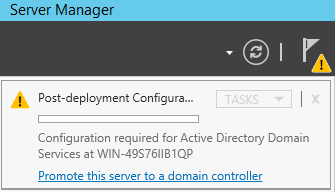
\includegraphics[width=.45\linewidth, height=.15\textheight]{PDC/install4}
\end{figure}
\item After your restart is complete you will see the above picture. Click on \textbf{Promote this server to Domain Controller}
\item The Deployment Configuration window will pop up.
\item Click the \textbf{Add a new forest}. Inside the root domain name text box, enter the domain name you wish to use followed by a period and the top level domain.(eg. .com, .ca, .local etc.)
\item In the Domain Controller Options window leave all values at the default except the password field.
\item Click next until you reach \textbf{Prerequisites Check}.
\item Verify all prerequisites have been met and click Install.
\end{enumerate}
\subsection{Domain Name System}
To set up DNS follow these steps:
\begin{enumerate}
\item In Server Manager Click \textbf{Tools} and then click \textbf{DNS}.
\item In the DNS Manager 
\begin{figure}[h]
	\centering
	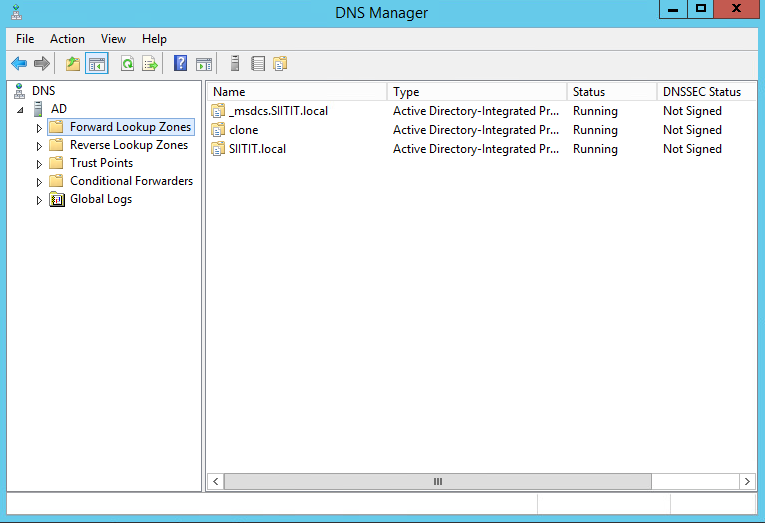
\includegraphics[width=0.6\linewidth]{dns/dns-install5}
\end{figure}
\item Here you can set up multiple domain zones. However if this is your initial domain controller setup you will see one domain available. You will see the domain you have previously created during the Active Directory setup.
\item When you click a zone you will be able to see all the hosts in that particular zone.
\item To add a host make sure you are inside the domain folder and right click the blank area. Click the \textbf{New A or AAAA host}
\item Make sure you have the \textbf{Create associated pointer} checked off to create the reverse lookup for that particular host.
\end{enumerate}
\newpage
\section{End Device Specifications}
Recording the specifications of host machines gives an idea of compatibility for the companies software and resources it requires.
\newline \newline
Shown below is one of the machines we have documented.
\begin{figure}[h]
	\centering
	\includegraphics[width=1\linewidth]{20180228_210547050_iOS}
\end{figure}
\begin{figure}
	\centering
	\includegraphics[width=1\linewidth]{"spec2 machine"}
\end{figure}
\newpage
\section{Creating the Clone Server}
The clone server is used to copy an existing machine and push it out to other machines. The purpose of cloning is to make it easier to produce copies of existing infrastructure. 
\subsection{Installing Disk-less Remote Boot For Linux}
Make a directory called images with the command \textbf{sudo mkdir /images} or another meaningful name to store your clone images. Next you want to give the directory root permissions using the \textbf{chown root:root /images} and \textbf{chmod 770 /images} to set permissions of read/write/execute to the user, group but not anyone else.\newline \newline
To add the key so that the clone server can obtain all of the required packages use:\newline\textbf{wget -q http://drbl.org/GPG-KEY-DRBL -0- | sudo apt-key-add -}
\newline
Go into superuser mode with \textbf{su} and use vi to get into the \textbf{/etc/apt/sources.list} file. 
\newline
You will need to add \textbf{deb http://free.nchc.org.tx/drbl-core drbl stable} to the end of the text file
\newline \textbf{Note:} You need to add the key and this line in order to download the full \textbf{DRBL} software when you run the \textbf{sudo apt-get update} command
\begin{figure}[h]
	\centering
	\includegraphics[width=1\linewidth]{"Screenshots-clone-server/Screenshot from 2018-03-10 13-33-36"}
\end{figure}
\newpage
\subsection{Configuring DRBL}
Update your system with \textbf{apt-get update}.
To install the clone server type \textbf{apt-get install drbl} after it is installed type in the command \textbf{apt-get install nmap} this ensures that DHCP can be run on the server. Once this is installed type in \textbf{drblpush -i}, the -i means it will run the program in interactive mode.\newline Any entry in this setup process in between [ ] is a default value. Pressing enter will use the value between these brackets, or enter your own to customize it to your network.
\begin{figure}[h]
	\centering
	\includegraphics[width=1\linewidth]{"Screenshots-clone-server/Screenshot from 2018-03-10 13-36-36"}
\end{figure}
\newpage
When you are on the step to set an initial value for the DRBL clients, pick a number that wont overlap with your existing static devices. For example if your network has host with an IP address of 172.16.6.8 it is best to set the initial client number to 15 in order to make sure no overlap exists.
\begin{figure}[h]
	\centering
	\includegraphics[width=1\linewidth]{"Screenshots-clone-server/Screenshot from 2018-03-10 13-39-10"}
\end{figure}
\newline
The next step will prompt you on the maximum amount of potential clients that will be assigned IP addresses.
\newline \newline
When you are asked which directory to store the cloned images on, use the folder created at \textbf{12.1}.
\begin{figure}[h]
	\centering
	\includegraphics[width=1\linewidth]{"Screenshots-clone-server/Screenshot from 2018-03-10 13-40-31"}
\end{figure} \newline
For a basic network setup you can leave the following settings as default, or else enter specific requirements tailored to your network.
\newpage
The next step you'll need to connect the server to the Internet then run \textbf{drblsrv -i}. Once it begins it will ask for values, leave them as their default values and select the kernel from this server. Once this is done you are ready for the next step.
\label{sec:12.2}
After running the drblsrv we are ready to start the clone server. To start the clone server type in \textbf{dcs}. You should see the screen shown below.
\newline \newline
Choose: \textbf{All Select all the clients}
\begin{figure}[h]
	\centering
	\includegraphics[width=1\linewidth]{"Screenshots-clone-server/Screenshot from 2018-03-10 13-51-18"}
\end{figure}
\newline
\textbf{Follow these steps for basic setup:}
\begin{enumerate}
	\item Clonezilla-start
	\item Beginner mode
	\item Save-disk
	\item Now in server
	\item Now choose a image name
	\item sda
	\item Skip checking (optional)
	\item -scs
	\item -p choose
	\item 1000000
\end{enumerate}
Once you have completed the previous steps start your client machine with Network Boot (F12 in most cases).
\newpage
\section{Preparing a system for Sysprep}
Before you can begin preparing sysprep you need to install Windows ADK. \href{https://go.microsoft.com/fwlink/p/?linkid=859206}{Download Here}
\newline

Mount a Windows 10 installation disc and copy the install.wim file in the sources folder to your desktop.
\begin{figure}[h]
	\centering
	\includegraphics[width=1\linewidth]{"sysprep/3-23-2018 13-23-45"}
\end{figure}
\newpage
\subsection{Configuring The Answer File}
Once installed open 'Windows System Image Manager'
\begin{figure}[h]
	\includegraphics[width=.5\linewidth]{"sysprep/3-23-2018 13-21-27"}
\end{figure}
Right click inside the Windows Image tab and click \textbf{Select Windows Image}
\begin{figure}[h]
	\includegraphics[width=.5\linewidth]{"sysprep/3-23-2018 13-48-20"}
	\includegraphics[width=.5\linewidth]{"sysprep/3-23-2018 13-25-37"}
\end{figure}
\newline Select the \textbf{install.wim} file we copied earlier.
\newline Next you will create a new answer file by clicking \textbf{New Answer File} in the file menu.
\begin{figure}[h]
	\centering
	\includegraphics[width=.5\linewidth]{"sysprep/3-23-2018 13-26-37"}
\end{figure}
\newpage
Under the \textbf{Components} tab right click \textbf{amd64\textunderscore Microsoft-Windows-Deployment} and add the setting to pass 4 specialize.
\begin{figure}[h]
	\includegraphics[width=1\linewidth]{"sysprep/3-23-2018 13-29-07"}
	\newline
	\textbf{Note:} Setting the Extend setting to \textbf{true} will automatically extend the partition to use up the entire hard-drive of the system you are cloning to.
	\includegraphics[width=1\linewidth]{"sysprep/3-23-2018 13-34-39"}
\end{figure}
\newpage
\begin{figure}[h]
	\includegraphics[width=1\linewidth]{"sysprep/3-23-2018 13-29-44"}
	\newline
	\textbf{Note:} Setting the \textbf{ComputerName} to \textbf{*} will automatically assign a unique identifier to each system when you run sysprep later on.
	\includegraphics[width=1\linewidth]{"sysprep/3-23-2018 13-35-03"}
\end{figure}
The \textbf{RegisteredOwner} will be a part of the computer name, we chose Student, however you can assign it with whichever identifier you want to use.
To set the \textbf{TimeZone} run the command \textbf{tzutil /g} in a CLI on Windows
\newpage
\begin{figure}[h]
	\centering
	\includegraphics[width=1\linewidth]{"sysprep/3-23-2018 13-32-46"}
\end{figure}

\begin{figure}[h]
	After adding in the OOBE into the Pass 7 oobesystem you will have to insert a new Local Account, doing so will allow you to set up a default Administrator account to the system automatically.
	
	\includegraphics[width=0.5\linewidth]{"sysprep/3-23-2018 13-36-14"}
	\includegraphics[width=0.5\linewidth]{"sysprep/3-23-2018 13-36-26"}
\end{figure}
\begin{figure}[h]
	\centering
	\includegraphics[width=1\linewidth]{"sysprep/3-23-2018 13-35-25"}
	After adding the \textbf{wow64\textunderscore Microsoft-Windows-International-Core neutral} set all the Locale to \textbf{en-US} or your preferred language.
\end{figure}
\newpage
Once you have setup the answer file save it to a portable thumb drive and copy it to the \textbf{C:\textbackslash Windows\textbackslash System32\textbackslash Sysprep\textbackslash} folder on the client machine you wish to clone
\newline

Next on the client machine run the CLI as an Administrator, doing so will put you into the \textbf{C:\textbackslash Windows\textbackslash System32} folder. The first command you will have to enter is \textbf{cd Sysprep} to enter into the Sysprep folder. Before this next step make sure you have everything setup on the computer you wish to copy over to all the other client machines. Once you are ready type in the command in the CLI:
\newline
\textbf{sysprep.exe /generalize /oobe /unattend:Unattend.xml /shutdown}
\newline
Once the computer has shutdown repeat the steps in \hyperref[sec:12.2]{12.2} using a different image name in step 5 as to not overwrite your previous image.
\newpage
\section{Multicast Cloning}
Multicast cloning gives you the ability to deploy an image from the server machine to all connected clients on the network. Using multicast cloning will cut down bandwidth usage on the network by sending out one packet that will replicate itself to clients on the specified list of MAC addresses.
\newline
Run the \textbf{dcs} command on the clone server and follow these steps:
\begin{enumerate}
	\item Clonezilla-start
	\item Beginner mode
	\item Restore-disk
	\item Skip checking (optional)
	\item -p choose
	\item Choose the image
	\item Select the disks you want to clone
	\item Multicast Multicast Restore
	\item Clients+time-to-wait
	\item Enter in how many clients you want to clone to
\end{enumerate}
After you have completed these steps now Network boot all the clients you want to clone.
\newline
\textbf{Note:} To network boot press the F12 key, this could be different depending on the machine hardware.
\section{Backup Domain Controller}
Once you have installed Windows Server 2012 on a backup machine, set a static IP address and DNS of the Primary Domain controller. 
\begin{figure}[h]
	\centering
	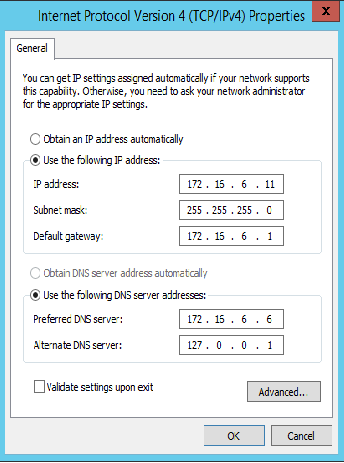
\includegraphics[width=0.35\linewidth, height=.35\textheight]{BDC/1}
\end{figure}
\newline \textbf{Note:} 127.0.0.1 is the localhost IP address of the local computer, set that as the alternate DNS server. You do this so that if the primary DNS goes down the backup DNS can take over.
\newpage Following the steps in \hyperref[sec:10.1]{10.1}, install the \textbf{Active Directory Domain Services} and the \textbf{DNS Server}. Once the installation is finished click \textbf{Promote this server to a domain controller}.
\begin{figure}[h]
	\centering
	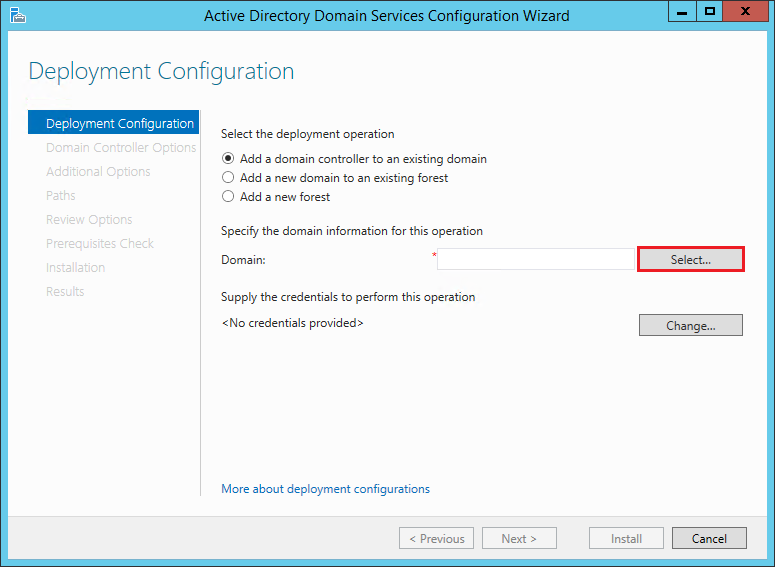
\includegraphics[width=.5\linewidth, height=.25\textheight]{BDC/1b}
\end{figure}

You have to set it to \textbf{Add to existing domain}. Then you enter the domain that you set up in the PDC. 
\newpage
\begin{figure}[h]
	\centering
	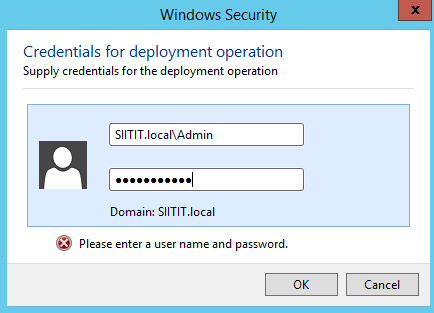
\includegraphics[width=.4\linewidth, height=.2\textheight]{BDC/2}
\end{figure}
Enter the Administrators credentials from the PDC in order for you to add the machine to the domain.
\begin{enumerate}
	\item In \textbf{Domain Controller Options} leave settings at their default except the \textbf{DSRM} password for recovery.
	\item Click next on the \textbf{DNS Options} unless you want to change any options for DNS.
	\item \textbf{Additional Options} make sure you replicate from the appropriate domain controller in your network.
	\item Click next until you are at the \textbf{Prerequisites Check} page, once all prerequisites have been met click on install.
\end{enumerate}
\section{Setting up Syslog}
Syslog receives logs from remotely connected devices in a network. With these logs you are able to troubleshoot and observe security information. These logs allow administrators to maintain the network properly by pinpointing flaws within the network.
\subsection{Installing A Syslog Server}
First you will have to install the Syslog server, we used Kiwi found at \href{https://www.kiwisyslog.com/free-tools/kiwi-free-syslog-server}{This website}
After downloading and installing Kiwi server \textbf{as a service}, on one your machines run the command \textbf{logging host (IP address of the server machine) eg. logging host 172.16.6.10} onto each of your routers. \textbf{Note:} Kiwi Free version only allows up to 5 connected devices.
\newpage
\section{Network Time Protocol}
Network Time protocol (NTP) is used to sync your internal network time to a single time server from the internet. The Canadian time servers are: 
\begin{enumerate}
	\item server 0.ca.pool.ntp.org
	\item server 1.ca.pool.ntp.org
	\item server 2.ca.pool.ntp.org
	\item server 3.ca.pool.ntp.org
\end{enumerate}
To setup the NTP connections enter in the following command on your backbone routers \textbf{ntp server (IP address/domain name) eg. ntp server 0.ca.pool.ntp.org}
\section{Access Control Lists}
Access control lists (ACLs) allow an administrator to control the flow of traffic within the network. With ACLs you can control the direction the traffic flows and restrict access by protocol, IP address, network. There are two types of ACLs; standard and extended. Standard ACLs are located near the destination while Extended ACLs are located near the source. ACLs are made up of one or more access control entries (ACEs). \textbf{All ACL have an explicit deny all applied to the end}
\newline

Standard ACL syntax:
\begin{enumerate}
	\item ip access-list standard (1-99 or a NAME)
	\item permit (IP address)
	\item permit (network address)
	\item int g0/0
	\item ip access-group (1-100 or a NAME) (IN or OUT)
\end{enumerate}

Extended ACL syntax:
\begin{enumerate}
	\item ip access-list extended (100-199,2000-2699 or a NAME)
	\item permit (protocol) (source) (destination) eq (port or name)
	\item int g0/0
	\item ip access-group (100-199, 2000-2699) (IN or OUT)
\end{enumerate}
\section{Virtual Local Area Network}
VLAN is a Virtual LAN that lets administrator restrict access to different areas of a network. Using VLANs administrator are able to enforce security policies, reduce the broadcast domains and traffic. VLANS are based on logical connection instead of physical connections.

\end{document}
